\documentclass{standalone}
\usepackage{tikz, tikz-cd}
\usetikzlibrary{shapes, decorations.markings}
\begin{document}

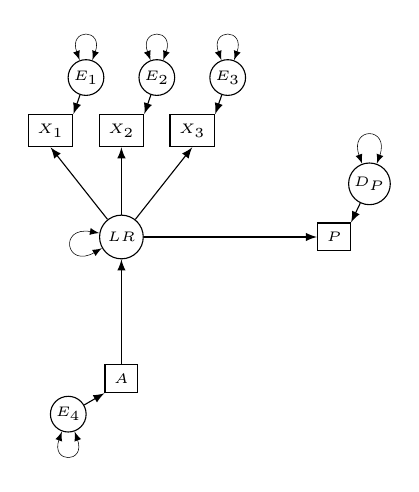
\begin{tikzpicture}[scale=0.9]
\node[draw] (o1) at (2,0) {\tiny{$A$}};
\node[draw, circle, inner sep=2] (l1) at (2,2) {\tiny{$LR$}};
\node[draw] (o2) at (1,3.5) {\tiny{$X_1$}};
\node[draw] (o3) at (2,3.5) {\tiny{$X_2$}};
\node[draw] (o4) at (3,3.5) {\tiny{$X_3$}};
\node[draw] (o5) at (5,2) {\tiny{$P$}};
\node[draw, circle, inner sep=1] (l2) at (1.5,4.25) {\tiny{$E_1$}};
\node[draw, circle, inner sep=1] (l3) at (2.5,4.25) {\tiny{$E_2$}};
\node[draw, circle, inner sep=1] (l4) at (3.5,4.25) {\tiny{$E_3$}};
\node[draw, circle, inner sep=1] (l5) at (1.25,-0.5) {\tiny{$E_4$}};
\node[draw, circle, inner sep=1] (l6) at (5.5,2.75) {\tiny{$D_P$}};
% Arrows
\draw [->, thin, >=latex] (l1)--(o2.south);
\draw [->, thin, >=latex] (l1)--(o3.south);
\draw [->, thin, >=latex] (l1)--(o4.south);
\draw [->, thin, >=latex] (l2)--(o2.north east);
\draw [->, thin, >=latex] (l3)--(o3.north east);
\draw [->, thin, >=latex] (l4)--(o4.north east);
\draw [->, thin, >=latex] (l5)--(o1.south west);
\draw [->, thin, >=latex] (o1)--(l1.south);
\draw [->, thin, >=latex] (l1.east)--(o5.west);
\draw [->, thin, >=latex] (l6)--(o5.north east);
% Residuals:
\draw[<->, very thin, >=latex] (l2) to [out=70,in=110,looseness=7] (l2);
\draw[<->, very thin, >=latex] (l3) to [out=70,in=110,looseness=7] (l3);
\draw[<->, very thin, >=latex] (l4) to [out=70,in=110,looseness=7] (l4);
\draw[<->, very thin, >=latex] (l5) to [out=250,in=290,looseness=7] (l5);
\draw[<->, very thin, >=latex] (l1) to [out=170,in=210,looseness=7] (l1);
\draw[<->, very thin, >=latex] (l6) to [out=70,in=110,looseness=7] (l6);
\end{tikzpicture}

\end{document}